\documentclass[11pt]{article}
\usepackage{algorithm2e}
\usepackage[bottom]{footmisc} 
\usepackage[italian]{babel}
\usepackage[document]{ragged2e}
\usepackage{tabularx}
\justifying
\usepackage{amsfonts, amssymb, amsmath}
\usepackage{cancel}
\usepackage{float}
\usepackage{mathtools}
\usepackage[margin=3cm]{geometry}
% \setcounter{secnumdepth}{0}
\usepackage{hyperref}
\hypersetup{
    colorlinks,
    citecolor=black,
    filecolor=black,
    linkcolor=black,
    urlcolor=black
}
\usepackage{array}
\usepackage{makecell}
\usepackage{hyperref}
\usepackage[noabbrev,capitalize,italian]{cleveref}
\newcommand{\fref}[1]{\hyperref[#1]{\cref{#1}}}
\usepackage{makecell}
\usepackage{etoolbox}
\patchcmd{\thebibliography}{\section*{\refname}}{}{}{}
\usepackage{enumitem}

\tolerance=1
\emergencystretch=\maxdimen
\hyphenpenalty=10000
\hbadness=10000

\begin{document}
\begin{titlepage}
    \begin{center}
        \vspace*{1.5cm}
            
        \Huge
        \textbf{Campionato di gare automobilistiche}
            
        \vspace{0.3cm}
        \LARGE
        Report\\[0.2em]

        \vspace{1.5cm}
          
        \begin{minipage}[t]{0.47\textwidth}
            \begin{center}
                \parbox{65mm}{\centering\large {\bf Cheikh Ibrahim $\cdot$ Zaid} \\[0.3em] Matricola: \texttt{0000974909} \\[0.3em] \href{mailto:zaid.cheikhibrahim@studio.unibo.it}{\textit{zaid.cheikhibrahim@studio.unibo.it}}} \\[2em]
            \end{center}
		\end{minipage}
		\hfill
		\begin{minipage}[t]{0.47\textwidth}\raggedleft
            \begin{center}
                \parbox{65mm}{\centering\large {\bf Xia $\cdot$ Tian Cheng} \\[0.3em] Matricola: \texttt{0000975129} \\[0.3em] \href{mailto:tiancheng.xia@studio.unibo.it}{\textit{tiancheng.xia@studio.unibo.it}}} \\[2em]
            \end{center}
		\end{minipage}  
            
        \vspace{9cm}
            
        Anno accademico\\
        $2022 - 2023$
            
        \vspace{0.8cm}
            
            
        \Large
        Corso di Basi di dati\\
        Alma Mater Studiorum $\cdot$ Università di Bologna\\
            
    \end{center}
\end{titlepage}
\pagebreak


\tableofcontents
\newpage


\section{Analisi dei requisiti}
\subsection{Requisiti espressi in linguaggio naturale \textbf{RIFRASARE IN FUTURO, E' GIUSTIFICATO IL TESTO?}}
Si vuole realizzare un database per gestire un campionato di gare automobilistiche. \\
È necessario codificare le gare, le piste su cui si svolgono, i dati relativi ai giri, eventuali infrazioni e i dati sui pit stop. \\
Inoltre, si vogliono memorizzare i dati dei piloti che partecipano e i contratti (presenti e passati) che stipulano con le scuderie. Oltre ai dati relativi alle scuderie, è richiesto registrarne le auto e i meccanici. \\
Infine, si vuole tenere traccia dei controlli di regolarità effettuati dai supervisori (della società che organizza il campionato) e dei dati degli sponsor delle gare e delle singole scuderie. \\[1em]

Per le gare si vuole memorizzare il nome, la data di svolgimento, la pista su cui si corre, il numero di giri previsti, i piloti partecipanti e l'eventuale sponsor. \\
Per le piste si vogliono rappresentare il nome, la nazione e la città di collocazione, la lunghezza (in metri), numero di posti a sedere per gli spettatori. \\
Per i giri si vogliono salvare il tempo impiegato (in secondi), il numero del giro, la gara di appartenenza, il pilota che effettua il giro. \\
Per le infrazioni si vogliono gestire i dati riguardanti il nome e la descrizione e vengono assegnate ad un giro di un pilota sottoforma di penalità (in secondi). \\
Per i pit stop si vogliono rappresentare il tempo delle operazioni, il tempo complessivo (tempo di entrata e uscita + tempo delle operazioni), il giro in cui viene il pilota che viene chiamato ai box e i meccanici che effettuano le operazioni. \\
Per i piloti si vogliono memorizzare il nome, cognome, luogo e data di nascita. \\
Per i contratti si vogliono rappresentare il numero identificativo, il pilota ed il suo numero identificativo, la scuderia, la data d'inizio e di fine, l'auto assegnata e il valore di ingaggio. \\
Per le scuderie si vogliono gestire i dati riguardo la ragione sociale, la nazione della sede principale, l'anno di fondazione, il colore caratterizzante e i vari sponsor. \\ 
Per le auto si vogliono salvare la potenza (in cavalli), velocità massima raggiungibile, la scuderia di appartenenza. \\
Per i meccanici si vogliono memorizzare il nome, cognome, luogo, data di nascita, il ruolo e la scuderia di appartenenza. \\
Per i controlli di regolarità si vogliono tracciare i dati riguardo la data e l'ora, l'auto coinvolta, il supervisore e l'esito. \\
Per i supervisori si vogliono memorizzare il nome, cognome, luogo, data di nascita. \\
Per gli sponsor si vogliono salvare la ragione sociale, la tipologia di azienda, il capitale investito e la nazione della sede principale.

\subsection{Glossario dei termini \textbf{RIVEDERE COLLEGAMENTI}}
\begin{tabularx}{\linewidth}{
        |>{\hsize=0.9\hsize}X|% 10% of 4\hsize 
        >{\hsize=1.8\hsize}X|% 30% of 4\hsize
        >{\hsize=0.6\hsize}X|% 30% of 4\hsize 
        >{\hsize=0.7\hsize}X|% 30% of 4\hsize
           % sum=4.0\hsize for 4 columns
    }
    \hline
    \textbf{Termine} & \textbf{Descrizione} & \textbf{Sinonimi} & \textbf{Collegamenti} \\
    \hline
    Società organizzante & Azienda che organizza un campionato & - & \\
    \hline
    Campionato & Numero definito di gare con classifica & - & Gare \\
    \hline
    Gare & Numero definito di giri & - & Piste, giri, piloti, sponsor \\
    \hline
    Giri & Percorrenza intera di una pista & - & Pilota, gara \\
    \hline
    Piste & Località asfaltata idonea al passaggio di veicoli ad elevata velocità & - & \\
    \hline
    Infrazioni & Eventi irregolari accaduti durante una gara & - & Penalità, giro, pilota \\
    \hline
    Penalità & Tempo ulteriore assegnato al tempo totale & - & \\
    \hline
    Auto & Autoveicolo ad elevata velocità & Veicolo & Scuderia \\
    \hline
    Piloti & Persona che guida un veicolo ad elevata velocità & - & \\
    \hline
    Scuderie & Azienda proprietaria di auto & - & Sponsor \\
    \hline
    Meccanici & Impiegati delle scuderie adibite alla manutenzione dell'auto & - & Scuderia \\
    \hline
    Supervisori & Impiegati della società organizzante adibiti ai controlli di regolarità & - & \\
    \hline
    Controlli (di regolarità) & Controlli effettuati dalla società organizzatrice per garantire la regolarità delle auto & Controlli & Supervisore \\
    \hline
    Sponsor & Azienda che investe per apparire in gare e/o in scuderie & - & \\
    \hline
    Pit stop & Fase di un giro dove l'auto sosta in un'apposita area di pista dove i meccanici effettuano operazioni all'auto & - & Giro, pilota, meccanici \\
    \hline
    Contratto & Accordo stipulato tra un pilota e una scuderia per gareggiare in un campionato & - & Pilota, scuderia \\
    \hline
\end{tabularx}    
\subsection{Eliminazione delle ambiguità presenti}
\subsection{Strutturazione dei requisiti}
\subsection{Specifica operazioni}

\section{Progettazione concettuale}

\subsection{Definizioni delle entità generali}
\begin{figure}[H]
    \centering
    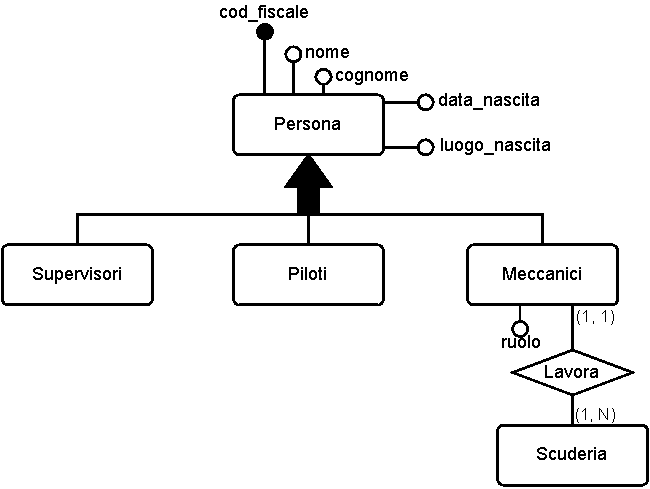
\includegraphics[width=11cm]{../er/gare_persone.pdf}
\end{figure}

\begin{figure}[H]
    \centering
    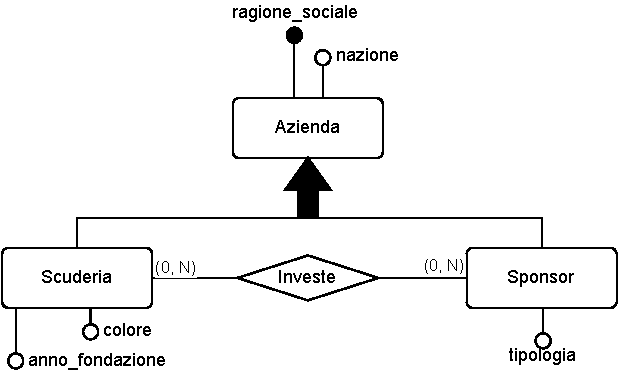
\includegraphics[width=11cm]{../er/gare_aziende.pdf}
\end{figure}

\begin{figure}[H]
    \centering
    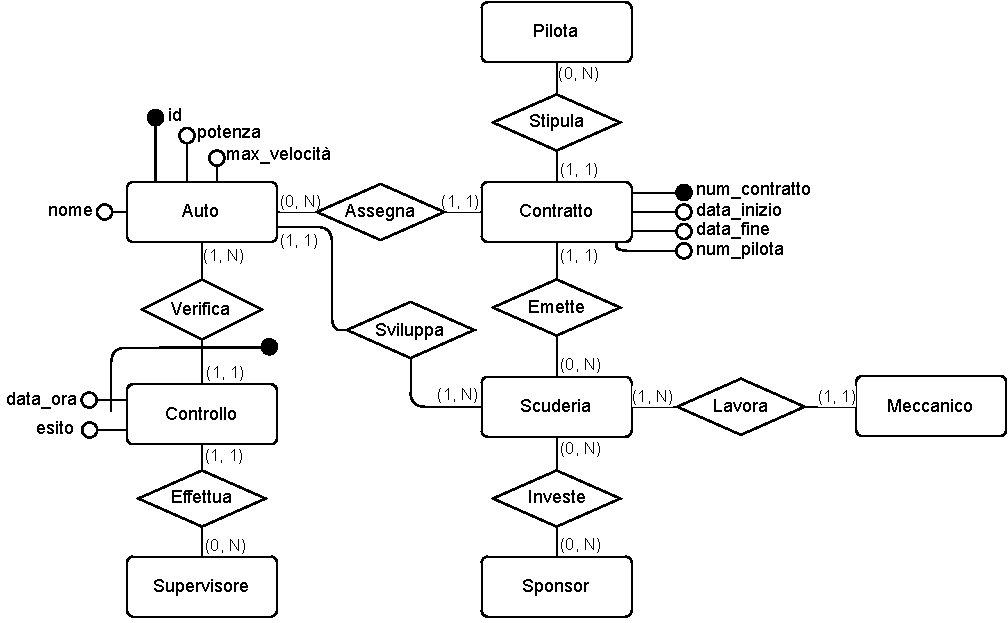
\includegraphics[width=15.5cm]{../er/gare_scuderie.pdf}
\end{figure}

\subsection{Identificazione delle entità e relazioni}
\subsection{Un primo scheletro dello schema}
\subsection{Sviluppo delle componenti dello scheletro}
\subsection{Unione delle componenti nello schema finale ridotto}
\subsection{Dizionario dei dati}
\subsection{Regole aziendali}

\section{Progettazione logica}
\subsection{Tavole dei volumi e delle operazioni}
\subsection{Ristrutturazione dello schema concettuale}
\subsection{Normalizzazione}
\subsection{Traduzione verso il modello relazionale}

\section{Codifica SQL}
\subsection{Definizione dello schema}
\subsection{Codifica delle operazioni}

\section{Testing}

\end{document}
